\rhead{Localization}


\chapter{Localization}
\label{sec:localization}

\begin{figure}[!h]
\centering
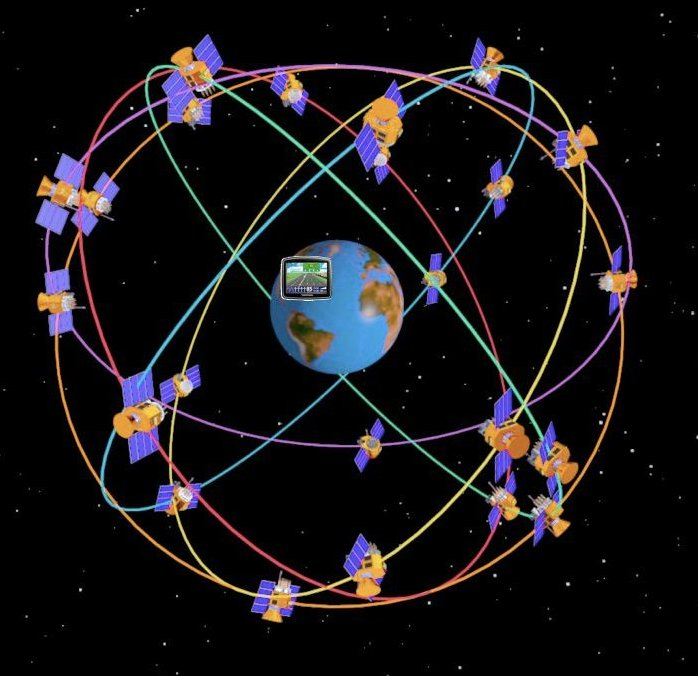
\includegraphics[width=0.9\columnwidth]{figures/8_teaser.jpg}
\end{figure}

\newpage

Without an external localization system, develop an autonomous robot controller using only on-board sensing and perception. 

\section{Introduction}

\vspace{0.5cm}
\noindent In the previous assignments, we have built up to a working robot soccer player.  You have developed an autonomous robot controller for 1-on-1 soccer using Player proxies for position control, bumper, and color blobfinding as well as our in-house overhead localization system.  Now it is time to remove the training wheels, specifically external top-down localization (this assignment) and internal state variables (next assignment).  

In the current assignment, you will implement a robot soccer controller that uses only the robot's on-board sensing and perception.  Specifically, you are only allowed to use Player's position2d, bumper, and blobfinding proxies.  With this perceptual information, you are tasked with implementing a localization system to determine your robot's pose on the pitch.  The pitch has been augmented with six color fiducials at the corners and midfield lines to facilitate your localization process.  These fiducials should be detectable using your object recognition code from Assignment 2.  Pose estimates from your localization, along with desired pose generation, will given to your {\bf working} path planning system from Assignment 3. 

\begin{figure}
\centerline{
\mbox{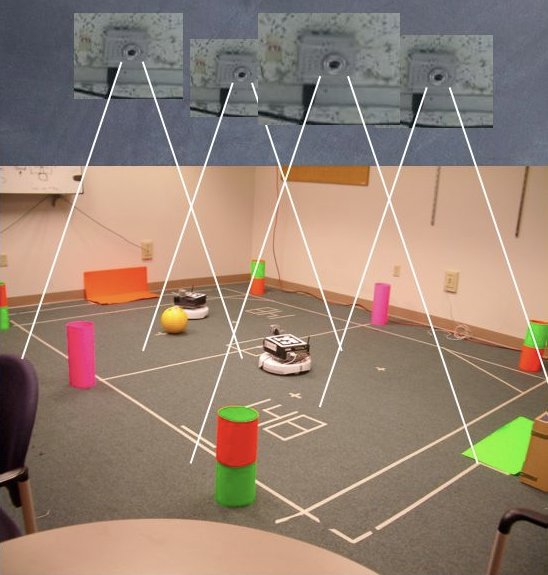
\includegraphics[width=3.44in]{figures/8_overhead_loc.jpg}}
\mbox{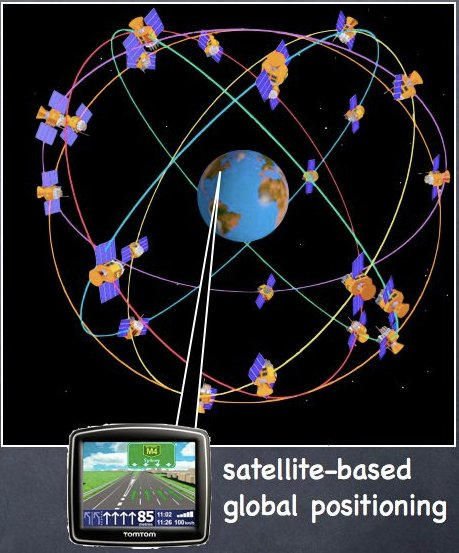
\includegraphics[width=3.00in]{figures/8_gps.jpg}}
}
\caption{Overhead Localization provided by overhead cameras or GPS}
\end{figure}

\section{Key Concepts}

\begin{figure}
\centerline{
\mbox{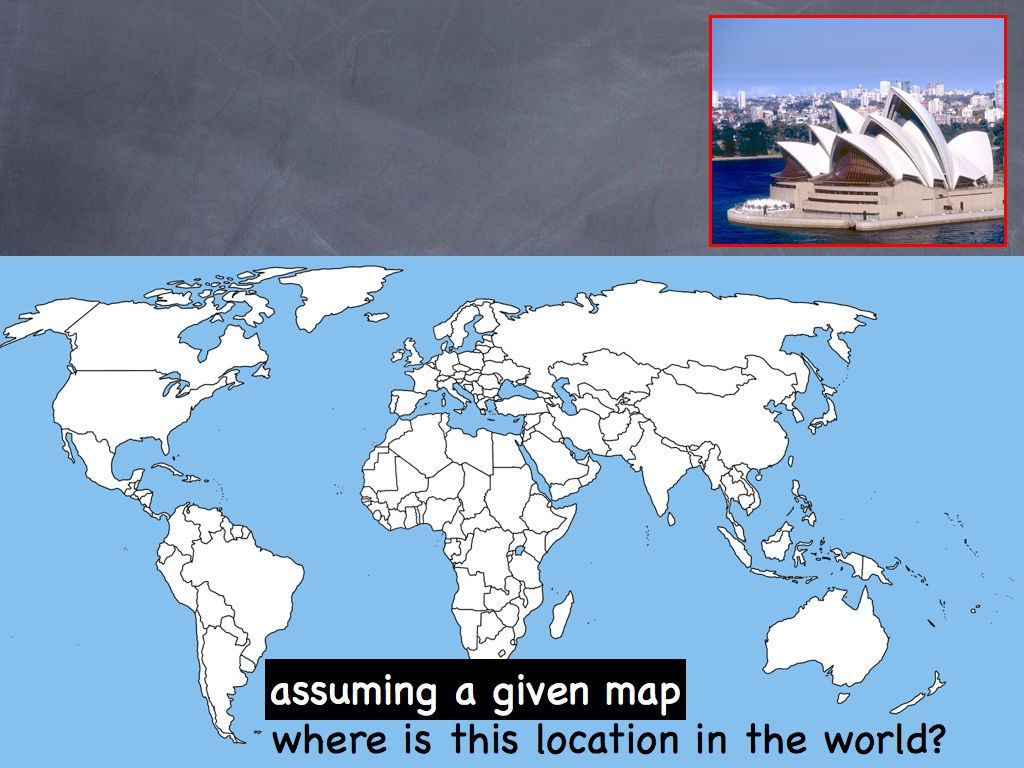
\includegraphics[width=3.20in]{figures/8_loc1.jpg}}
\mbox{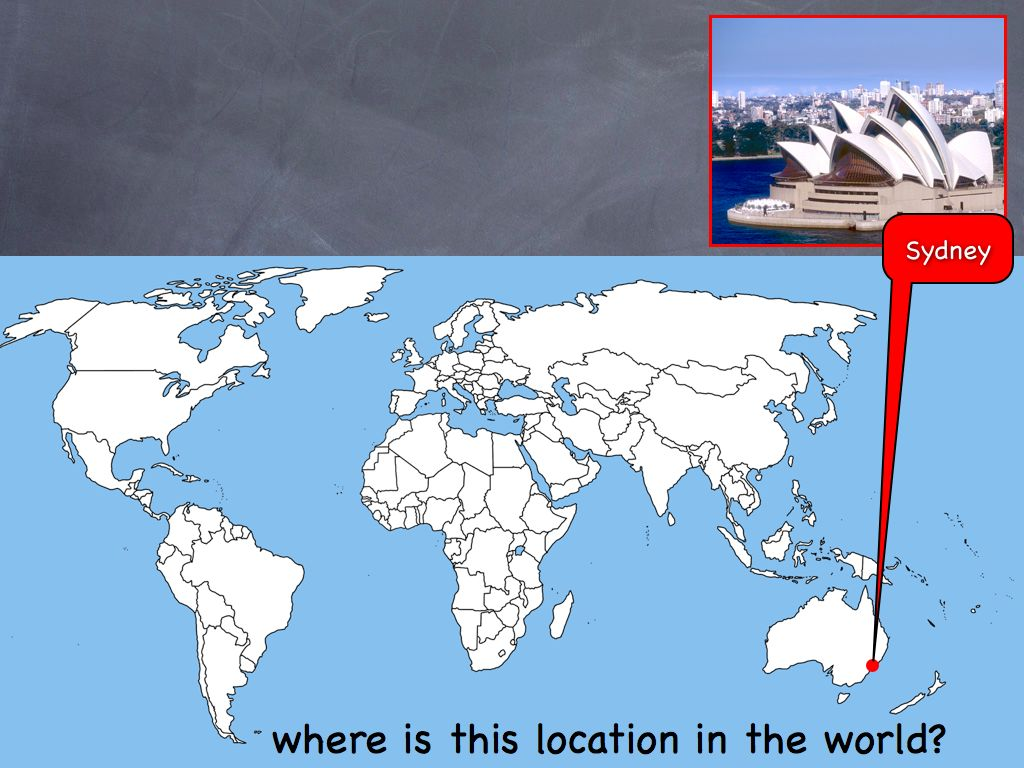
\includegraphics[width=3.20in]{figures/8_loc2.jpg}}
}
\end{figure}

\begin{figure}
\centerline{
\mbox{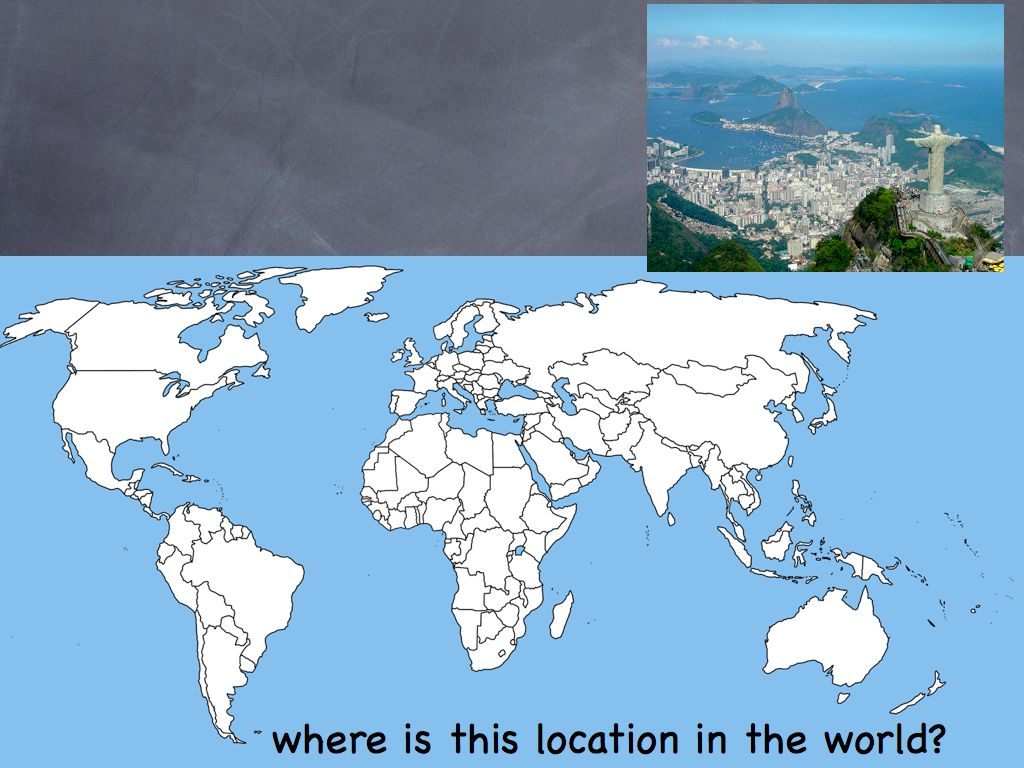
\includegraphics[width=3.20in]{figures/8_loc3.jpg}}
\mbox{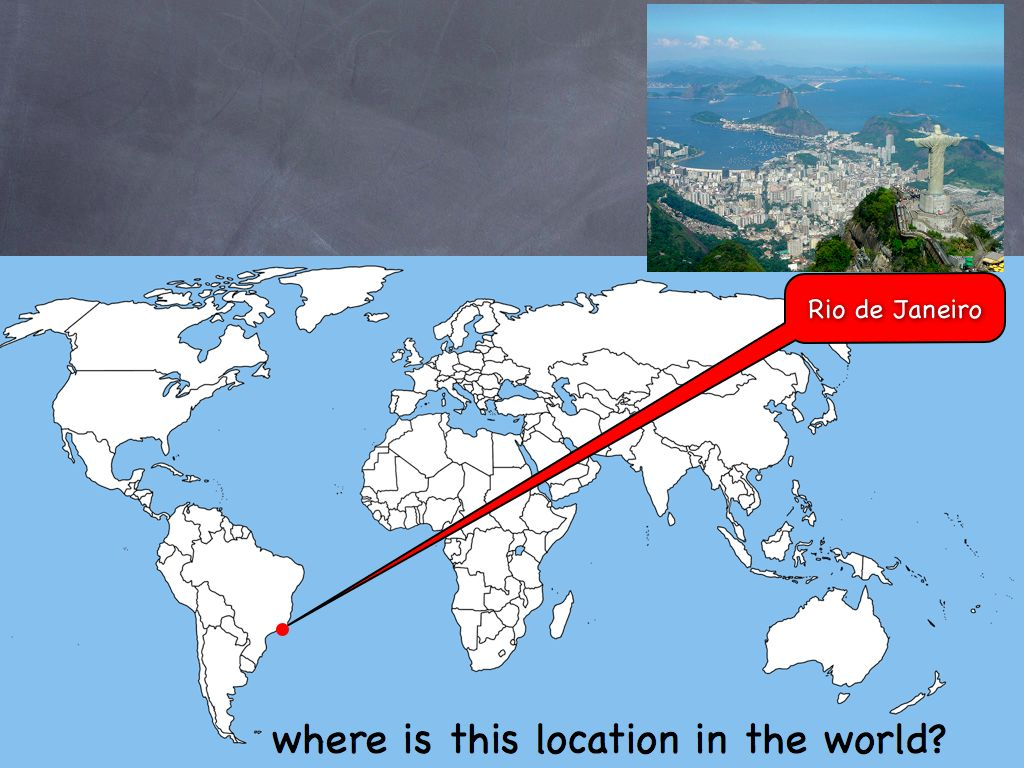
\includegraphics[width=3.20in]{figures/8_loc4.jpg}}
}
\end{figure}

\begin{figure}
\centerline{
\mbox{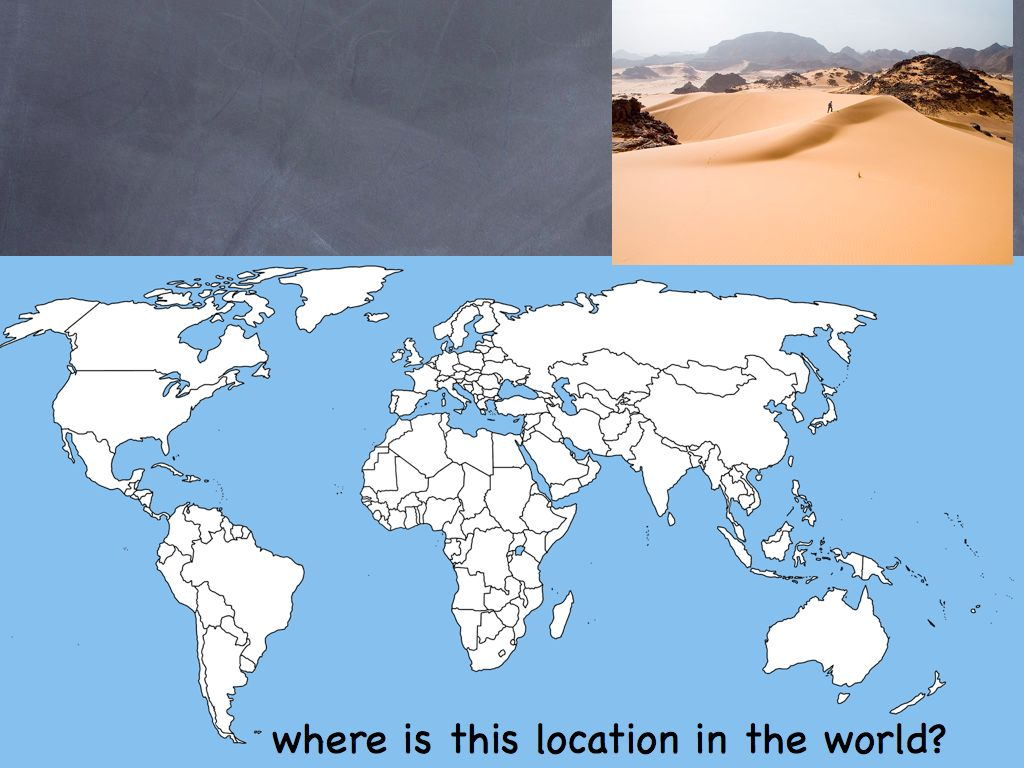
\includegraphics[width=3.20in]{figures/8_loc5.jpg}}
\mbox{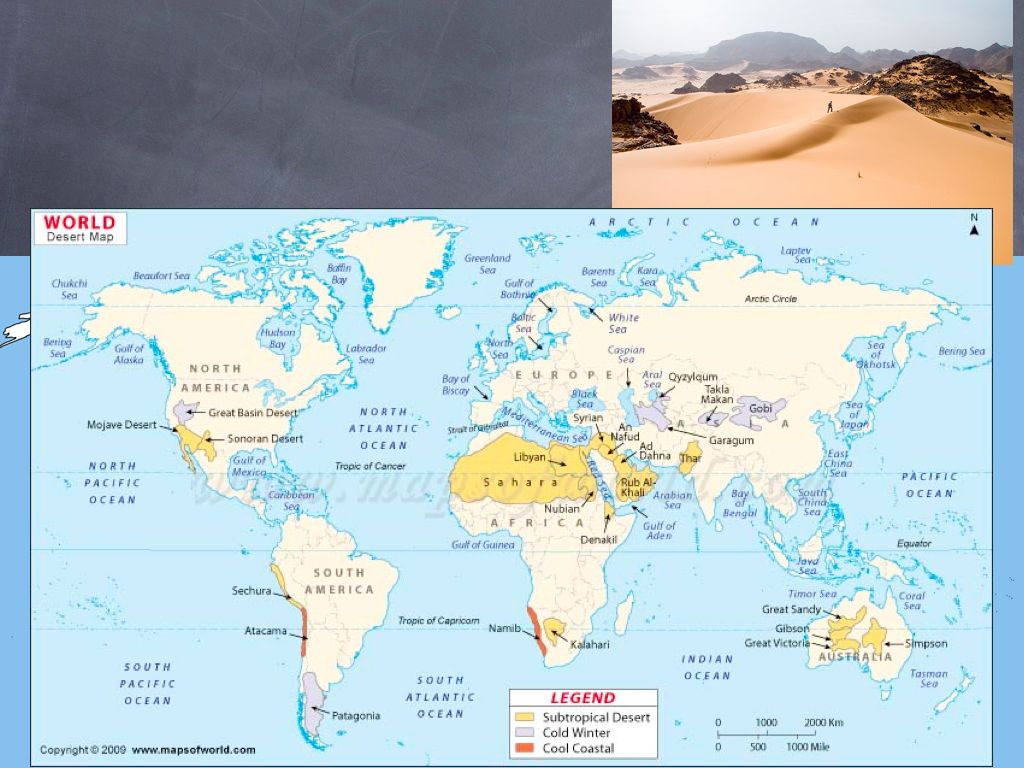
\includegraphics[width=3.20in]{figures/8_loc6.jpg}}
}
\end{figure}


\begin{figure}
\centerline{
\mbox{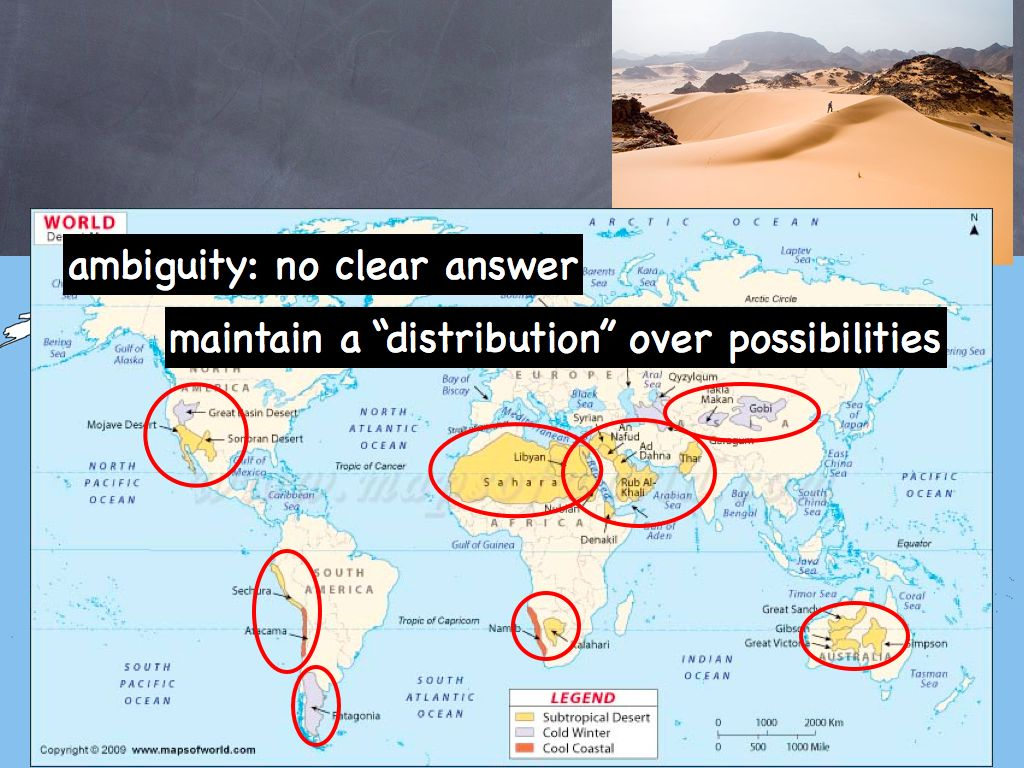
\includegraphics[width=3.20in]{figures/8_loc7.jpg}}
}
\end{figure}


\begin{figure}
\centerline{
\mbox{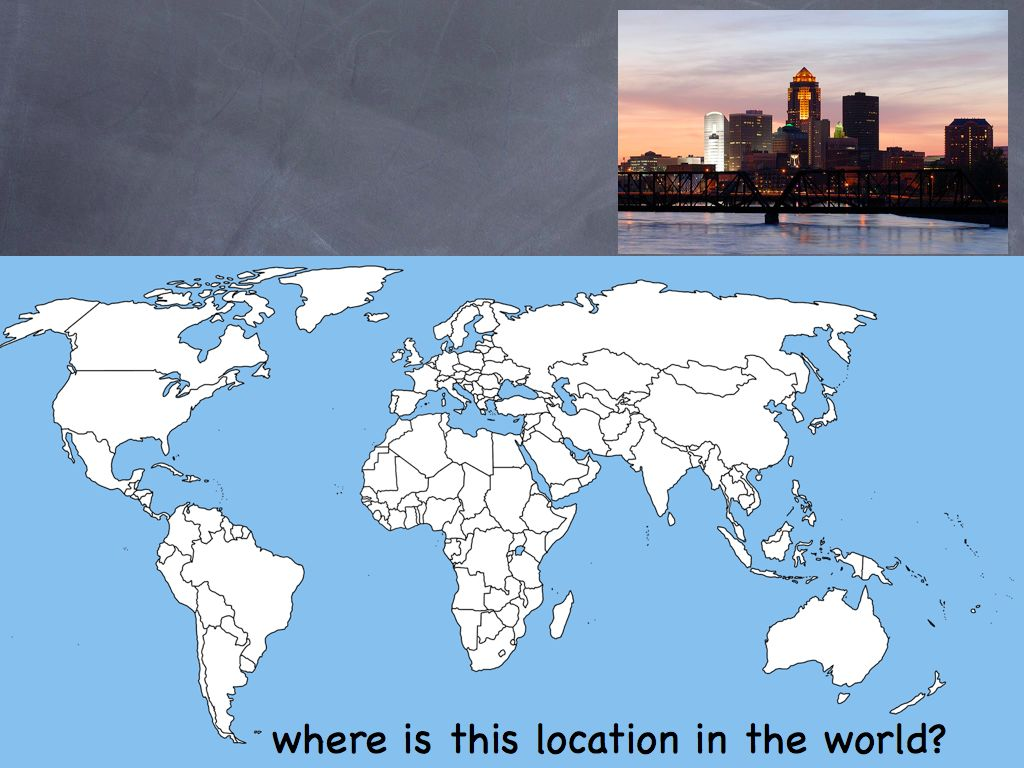
\includegraphics[width=3.20in]{figures/8_loc8.jpg}}
\mbox{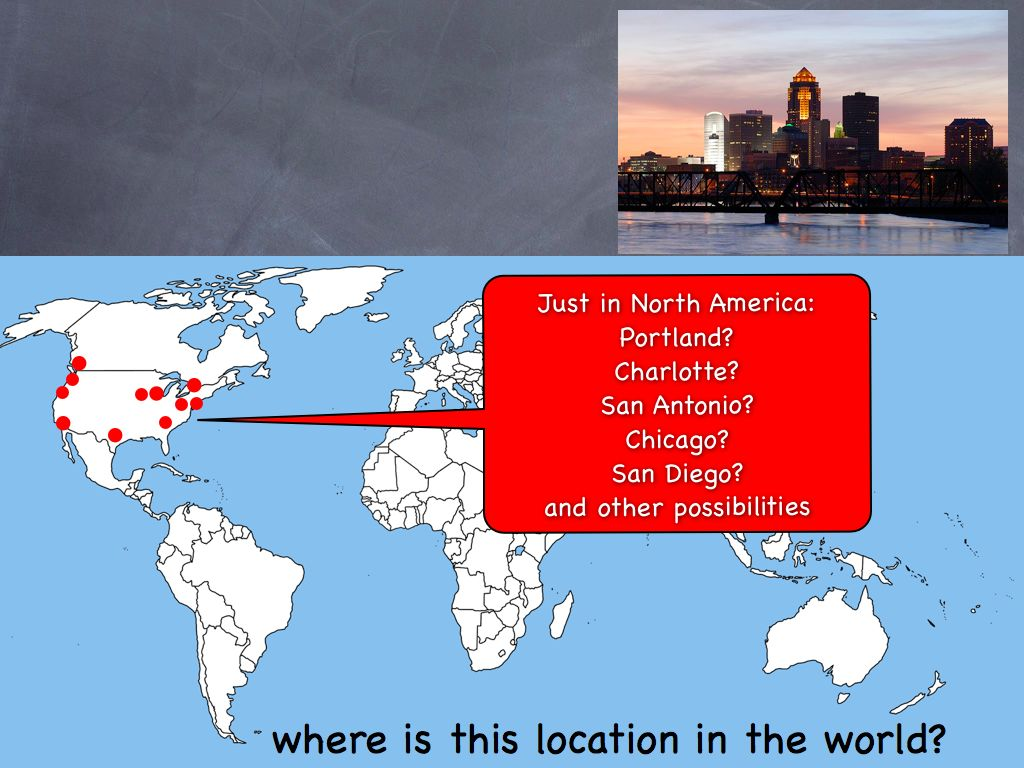
\includegraphics[width=3.20in]{figures/8_loc9.jpg}}
}
\end{figure}

\begin{figure}
\centerline{
\mbox{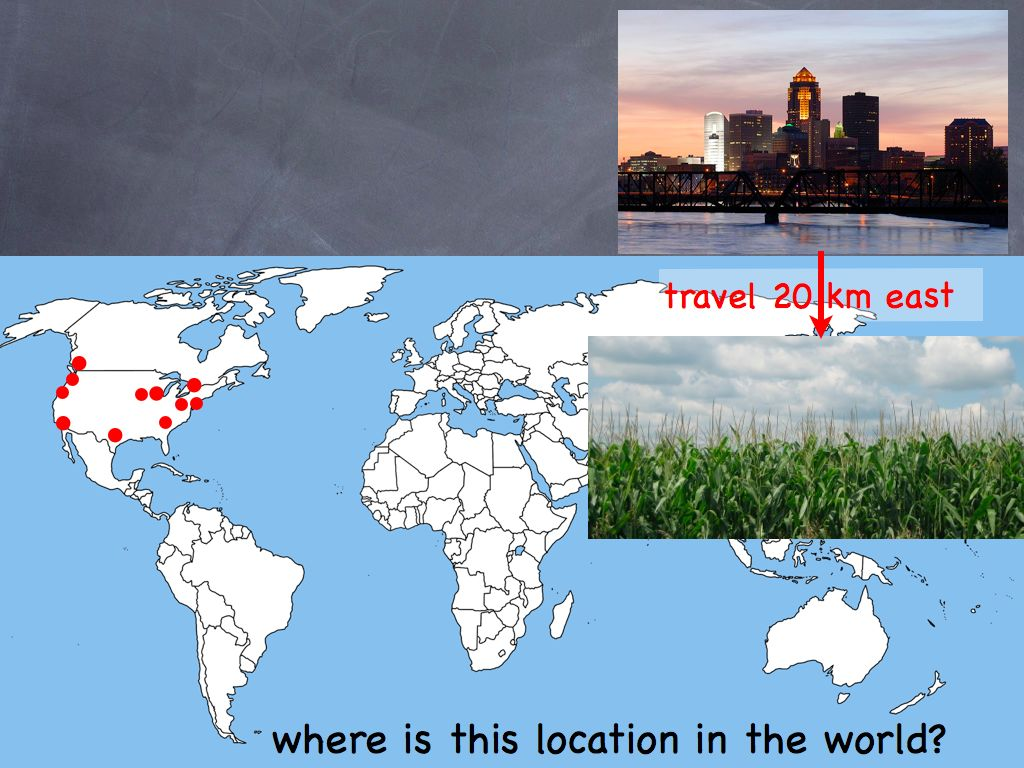
\includegraphics[width=3.20in]{figures/8_loc10.jpg}}
\mbox{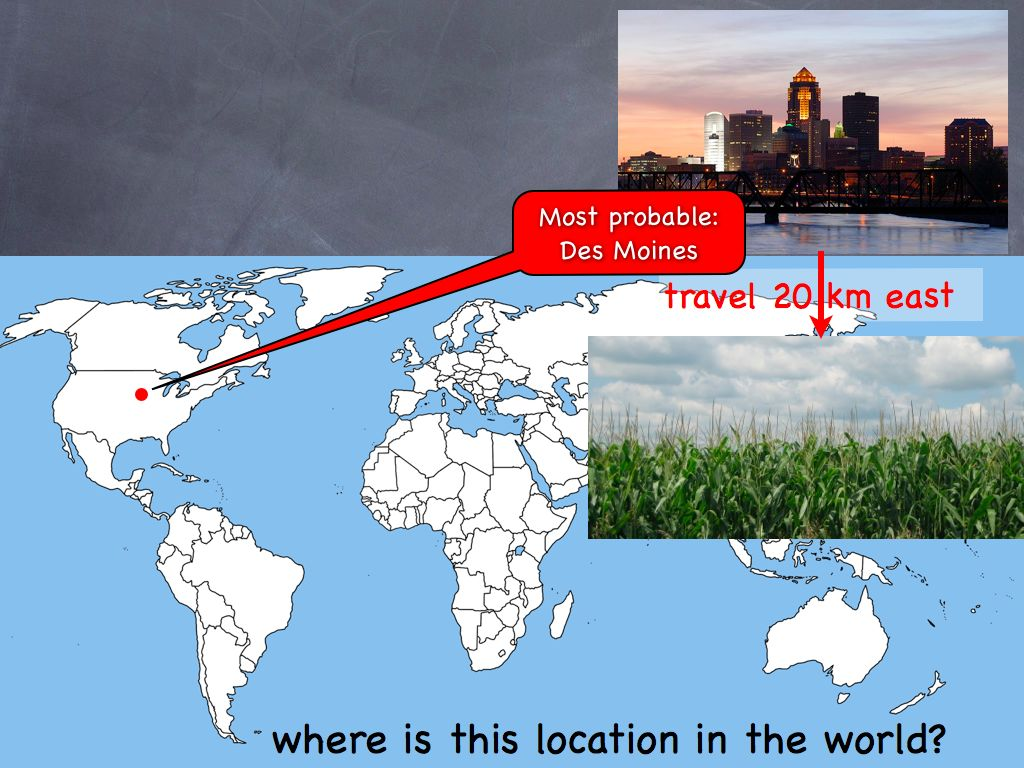
\includegraphics[width=3.20in]{figures/8_loc11.jpg}}
}
\end{figure}


\subsection{Particle Filter}

link: Particle Filter Matlab Demo

\subsection{Kalman Filter}

link: Kalman Filter Matlab Demo

\subsection{Probabilistic Measurement Model}

A tutorial on the landmark measurement model used for the localization assignment.

\textbf{TODO: include Jonas' paper on probabilistic measure model}

\section{Project Infrastructure}

\section{Instructions}

For this project, your client will continually estimate the current pose of your robot to enable path planning.  Your localization system must be able to estimate the probablity of the robot being in a certain pose $X = (x,y,\theta)$ given your current perception values $Z$ given by odometry, object recognition, and bumper and a known map.  The map will contain the locations of relevant objects, namely goals and fiducials.  Your existing path planner will use this pose estimate to generate a path on the field to traverse.

In class, we have covered several different localization algorithms based on the Bayes filter\footnote{\href{http://en.wikipedia.org/wiki/Recursive_Bayesian_estimation}{refer to Wikipedia entry on ``Recursive Bayesian estimation''}}:

\begin{equation}
p(X_{t}|Z_{t}) \propto p(Z_{t}|X_{t}) \sum_{X_t} p(X_{t}|X_{t-1}) p(X_{t-1}|Z_{t-1})
\end{equation}

which, roughly stated, generates the robot's new location belief at time $t$, or {\it posterior} $p(X_{t}|Z_{t})$, by using its old belief at time $t-1$, or {\it prior} $p(X_{t-1}|Z_{t-1})$ to predict a new belief, or {\it dynamics} $p(X_{t}|X_{t-1})$, that is matched against reality, or {\it likelihood} $p(Z_{t}|X_{t})$.  Several algorithms can be used to perform filtering for localization:

\begin{itemize}
\item Filtering with grid-based discretization
\item Kalman filtering: Markovian linear dynamics with parametric Gaussian-distributed unimodal noise 
\item Particle filtering: probablistic Markovian dynamics with nonparametric noise distributions and importance sampling
\end{itemize}

However, you will find that defining proper likelihood and dynamics terms are not explicitly covered by the algorithms.  Specifically, your dynamics should use odometric information about the robot's pose given by Player's position2d proxy.  Your likelihood function should evaluate the plausibility of perceiving information from the blobfinder and bumper proxies given a hypothesis that you are in a particular pose.  You will spend some time and careful consideration in defining these terms.  

Additionally, you will need to consider how to extract a single localization decision if you have a multi-modal posterior distribution.  As discussed in class, {\it maximum a posteriori} (maximum), expectation (mean), and robust mean are options for extracting such pose estimates.

{\bf Active localization:} It should be noted that your decision making can help resolve ambiguity for your localiztion system.  That is, you can decide to move your robot towards locations that would make its location more clear.

\begin{figure}
\centering
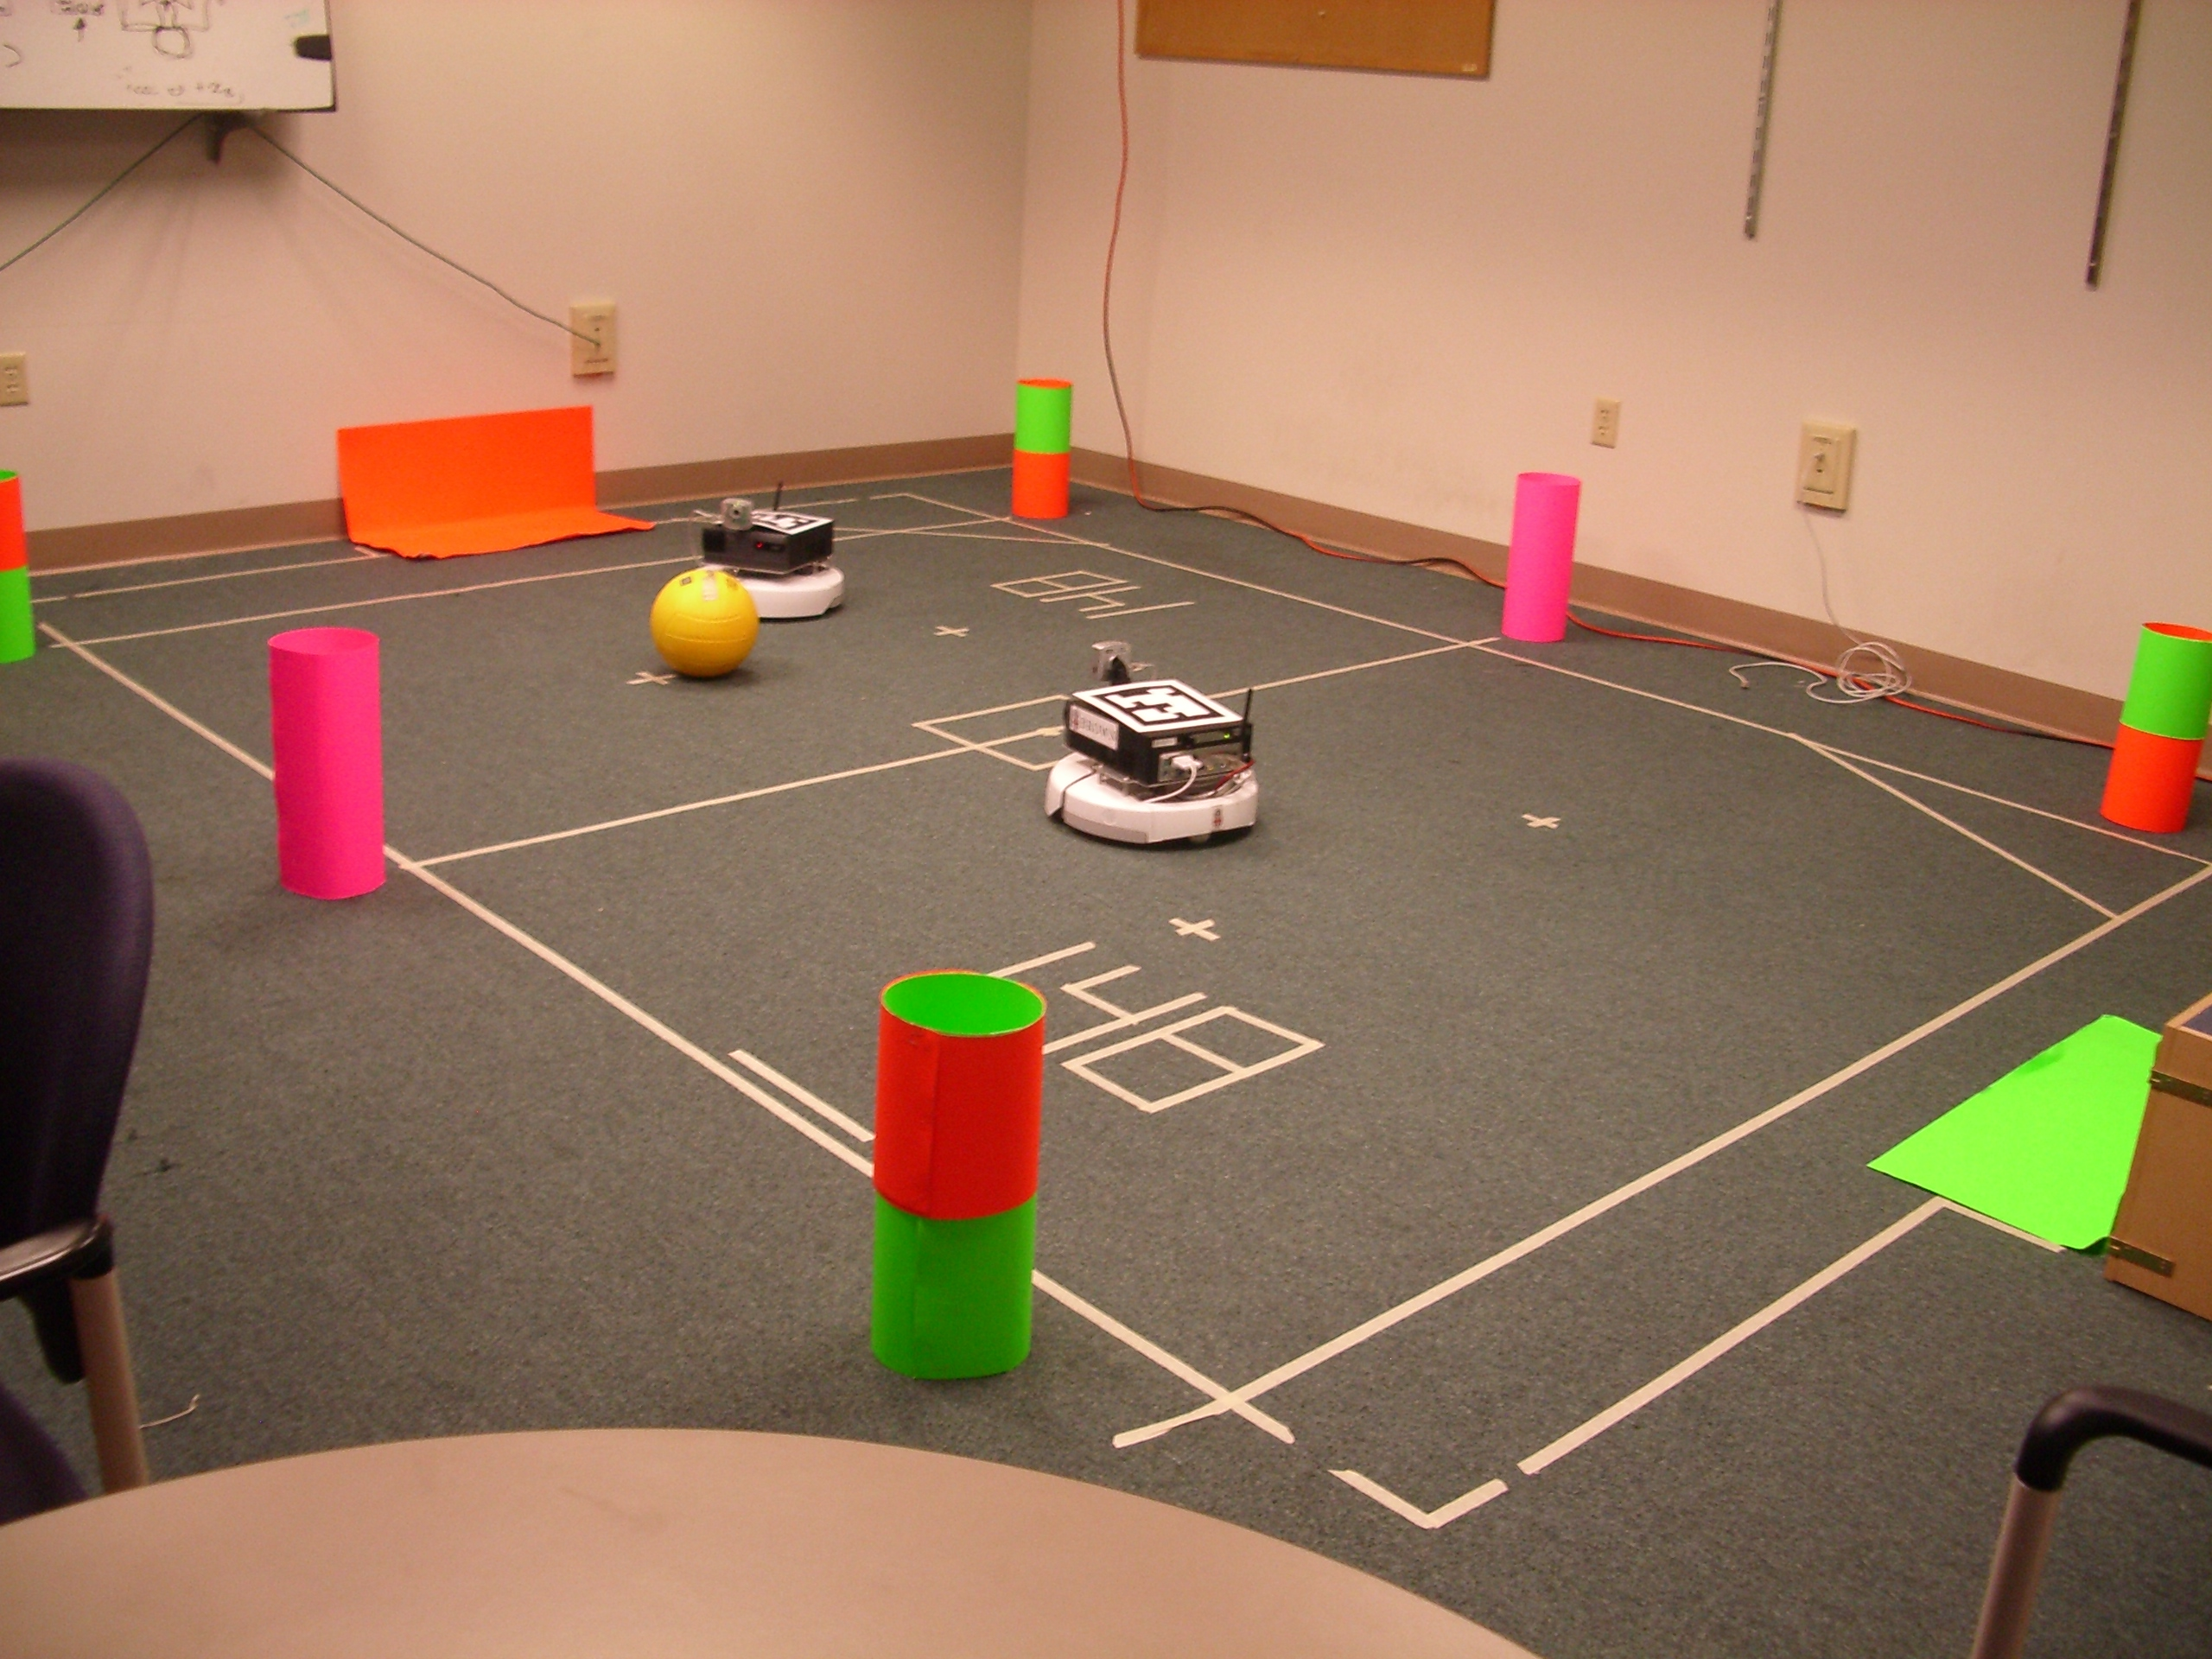
\includegraphics[width=0.7\textwidth]{figures/8_field.jpg}
\vspace{0.5cm}
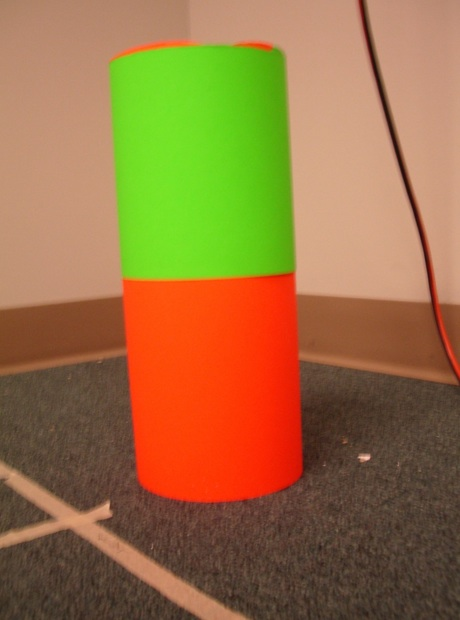
\includegraphics[width=.35\textwidth]{figures/8_cornerr.jpg}
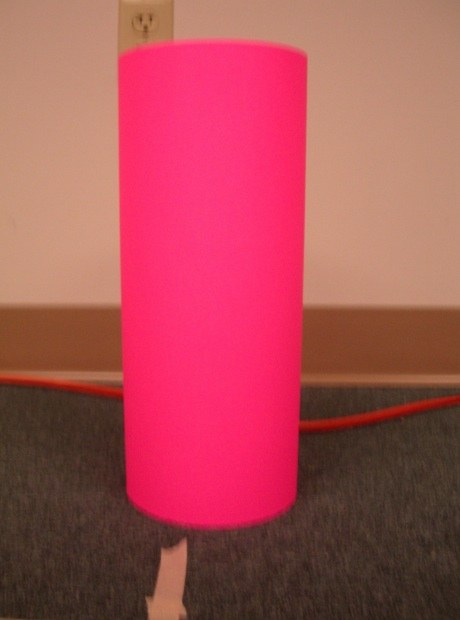
\includegraphics[width=.35\textwidth]{figures/8_midfieldr.jpg}
\caption{Snapshot of the ``FC 148'' robot soccer field with fiducial landmarks at the corners (such as ``green'' over ``orange'') and midfield line (as ``pink''). }
\label{fig:field}
\end{figure}

\textbf{Desired Pose Determination}

Also, you are not restricted to using only your path planner for decision making, but it is highly recommended.  At the very least, you should consider using some combination of your planner and other control heuristics.

In addition to estimating the current pose of your robot, you will also need to determine desired poses for your path planning system.  Your calculation of desired pose can (and probably should) use estimates of your robot's pose along with recognition of the ball.  It is not necessary to perform localization on the ball's location, but this is not necessarily a bad idea.  You may want to try to estimate the depth of the ball from blob dimensions, which is (again) not necessary.  Note: the ball will not be occluded during the skills challenges, but may be occluded during gameplay due to the other player.

Given our current soccer setup, localization of the other player will be difficult and is discouraged. 


\section{Expected Outcomes and Reports}

\vspace{1cm}
\begin{tabular}{|l|l||l|l|}
\hline
{\large \bf Project Implementation} & \\
\hline
\hline
Localization & 30\% \\
$\rightarrow$ Does your robot properly estimate its location? & \\
$\rightarrow$ Does this estimate account for uncertainty and ambiguity in perception? & \\
\hline
Goal Attainment  & 10\% \\
$\rightarrow$ Can your robot drive to a given sequence of locations on the field? & \\
$\rightarrow$ Can the robot avoid given unseen regions on the pitch? & \\
\hline
Soccer Proficiency & 5\% \\
$\rightarrow$ How well does your robot player soccer in the given environment? & \\
\hline
Controller Robustness & 5\% \\
$\rightarrow$ Does your controller run without interruption? & \\
\hline
\end{tabular}

\newpage
